
\chapter{Two key ML principles}
\index{bias-variance trade-off}

\section{``The bias-variance trade-off''}

Earlier in the book (p.~\pageref{bvTradeoffLowess}) I made a reference to
something called ``the bias-variance trade-off.'' This turns out to be one of
the most important general principles in all of ML, and it's now time to look
at it in detail.

\index{no free lunch@the ``no free lunch'' principle}

The \textbf{bias-variance trade-off} is a manifestation of the ``no free
lunch'' principle. Classifiers that possess one advantage inherently have a
counteracting disadvantage. Here are the two key terms:

\begin{itemize}
\itemsep.1em

\item \textbf{bias}\footnote{Tip: when thinking about this topic, try to erase
your previous definitions for the word ``\textit{bias}'' that you have running
around in your brain. They probably don't apply. The normal meaning of the word
``bias'' implies a systematic propensity to err \textit{in a particular
direction}. Like, ``you're biased towards thinking people are shorter than they
are, because you're tall.'' But in this chapter, \textit{bias} just means
``being `off' in general, in whatever direction, and probably not the same
direction each time.''} -- the degree to which a model is expected to
misclassify items, even those in its own training set, because it just can't
``bend'' enough to catch every data point.

\item \textbf{variance} -- the degree to which a model will differ based on the
particular training set that is chosen, because it ``bends'' too much to try
and catch every data point.

\end{itemize}

\index{Sith}
\index{Jedi}
\index{security camera}
\index{spycam}

The basic theory is as follows. Suppose you have a very simple classifier that
takes 714 training points from a security camera and tries to identify a
single, smooth, perfectly straight line roughly separating Jedi from Sith.
Maybe our model says ``just use the \texttt{lightsaber} feature by itself, and
call `\texttt{Jedi}' or `\texttt{Sith}' based on whether the test point's
lightsaber value is more typical of the \texttt{Jedi} Knights or the
\texttt{Sith} Lords in the training set.''

This simple classifier can be said to have \textbf{low variance}. Why? Because
if, instead of those particular 714 training points chosen from the
population, I had sampled a different 714 training points, \textit{the
classification decisions I would make on new data would be about the same.} To
see why this is the case, consider how different the training sets would have
to be in order for me to make any \textit{different} decisions. Let's say the
lightsaber colors for my original 714 training points were:

\label{simpleClassifierTable}
\Large
\begin{center}
\begin{tabular}{|l|rr|}
\hline
& Jedi & Sith \\
\hline
red & 17 & 85 \\
blue & 283 & 28 \\
green & 299 & 2 \\
\hline
\end{tabular}
\end{center}
\normalsize

Clearly, my very simply classifier is going to predict \texttt{Sith} for
\texttt{red}-lightsaber wielders and \texttt{Jedi} for anyone else. Now if I
had collected a different training set, the numbers above would be different,
but they would have to be a \textit{lot} different to change any of my future
predictions. I'd have to have an additional 68 \texttt{red} \texttt{Jedi}, for
instance, or 255 additional \texttt{blue} \texttt{Sith}, or a whopping 297
additional \texttt{green} \texttt{Sith}. Not likely.

That's the bright side. On the dark side, by classifying points in this way,
this simple model is going to get a lot of data points wrong: $17+28+2=47$
points incorrect \textit{in its own training set}, in fact. This mean it's a
pretty \textbf{high bias} classifier.

It's a tradeoff. In exchange for being virtually immune to the idiosyncrasies
in the training sample, we've sacrificed some precision.

\index{kNN@kNN ($k$-nearest neighbors)}

The other extreme can be seen by visualizing a 1-NN classifier. When given a
new data point, 1-NN will find the \textit{single} nearest neighbor to it in
the training set, and call \texttt{Jedi} or \texttt{Sith} accordingly. This is
very \textbf{low bias} -- heck, we're guaranteed to get every training point
correct! \footnote{Think about it: if we go through the training points one by
one, and treat them as new points, the ``nearest neighbor'' to each one will be
itself! (Unless there are data points with identical feature values but
different labels, in which case whatcha gonna do.)} But it is also very
\textbf{high variance}: swap out the training set for another, and you'll get
many, many different classifications. Our classifier has essentially memorized
a zillion individual examples, and will regurgitate all that intricate detail
on command. But had we gotten a different random sample, the ``single nearest
neighbor'' to a test point would have been totally different, and might result
in a different classification.
     
\subsection{``Overfitting''}

\index{overfitting}
\index{data-generating process (DGP)}

Another very important term to learn here is the word ``\textbf{overfitting}.''
That's what our 1-NN classifier is doing. When a model is overfitting, it means
that it is allowing itself to be ``too flexible'' in its quest to bend exactly
to its training points. It thus gets hyper-calibrated to a particular training
set. Instead of locking on to the true, general, repeatable patterns of the
underlying data-generating process, it's locking on to whatever idiosyncrasies
were present in the particular data points it was given. And this will almost
always lead to bad performance on new data.

There are formulas you can use to work out quantitatively what the estimated
bias and variance are for a classifier. But I think this dichotomy is more
important from a conceptual perspective. The main lesson is: the more your
classifier ``bends'' (\textit{i.e.}, has a very wiggly and flexible boundary
between its ranges of predicted values) the more precise it potentially is in
selectively labeling data points. However, this also means that a lot of its
decisions are going to hinge on the particular data sample it was trained on,
which means it will probably be overfitting: picking up noise in addition to
signal.

\subsection{kNN vs.~Na\"{i}ve Bayes}

Let's compare how 3-NN and Na\"{i}ve Bayes perform on these two dimensions.
Figure~\ref{comparisonCode} at the end of the chapter
(p.~\pageref{comparisonCode}) defines two functions. One runs a Na\"{i}ve Bayes
classifier on a security camera data set, using a random sample of 70\% for
training, and returns the percentage of the test set that it gets correct. The
other does the same for a kNN classifier (its second parameter is the value of
\texttt{k}.)

We can then run the following code to test each classifier on 200 different
random training sets:

\index{facetgrid@\texttt{FacetGrid()} (Seaborn)}
\index{facets}
\index{melt@\texttt{melt()} (Pandas)}

\begin{Verbatim}[fontsize=\footnotesize,samepage=true,frame=single,framesep=3mm]
nb_performances = np.empty(200)
for i in range(200):
    nb_performances[i] = naive_bayes(s)

knn_performances = np.empty(200)
for i in range(200):
    knn_performances[i] = kNN(s, 3)

results = pd.DataFrame({'Naive Bayes':nb_performances, '3-NN':knn_performances})
results_l = pd.melt(results, [], var_name='classifier', value_name='accuracy')
facet = sns.FacetGrid(results_l, col='classifier')
facet.map(plt.hist, 'accuracy', bins=20)
\end{Verbatim}

\begin{figure}[ht]
\centering
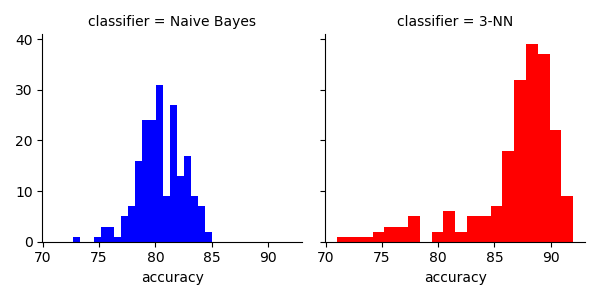
\includegraphics[width=0.9\textwidth]{nb_knn_comparison.png}
\caption{The accuracies of Na\"{i}ve Bayes and 3-NN classifiers, on 200
different training sets.}
\label{nb_knn_comparison}
\end{figure}

The result is shown in Figure~\ref{nb_knn_comparison}. It is very revealing.
First, notice that on average, the 3-NN classifier beats Na\"{i}ve Bayes. The
mean accuracies are:

\begin{Verbatim}[fontsize=\footnotesize,samepage=true,frame=single,framesep=3mm]
print("Naive Bayes: mean accuracy {:.2f}%.".format(nb_performances.mean()))
print("3-NN: mean accuracy {:.2f}%.".format(knn_performances.mean()))
\end{Verbatim}
\vspace{-.2in}

\begin{Verbatim}[fontsize=\footnotesize,samepage=true,frame=leftline,framesep=5mm,framerule=1mm]
Naive Bayes: mean accuracy 80.47%.
3-NN: mean accuracy 86.81%.
\end{Verbatim}

This tells us that 3-NN has \textbf{lower bias}, which is a good thing: good
enough for another 6\%-ish prediction accuracy, in fact.

The second thing to notice, though, is that the performance of 3-NN is more
variable. Its range is from 70-92, as opposed to Na\"{i}ve Bayes' 73-85. This
means that on some training sets, its performance is actually lower than the
worst of any of the Na\"{i}ve Bayes runs. The standard deviation bears this
out:

\begin{Verbatim}[fontsize=\footnotesize,samepage=true,frame=single,framesep=3mm]
print("Naive Bayes: standard deviation {:.2f}.".format(nb_performances.std()))
print("3-NN: standard deviation {:.2f}.".format(knn_performances.std()))
\end{Verbatim}
\vspace{-.2in}

\begin{Verbatim}[fontsize=\footnotesize,samepage=true,frame=leftline,framesep=5mm,framerule=1mm]
Naive Bayes: standard deviation 2.04.
3-NN: standard deviation 4.07.
\end{Verbatim}

\index{no free lunch@the ``no free lunch'' principle}

So 3-NN has \textbf{higher variance}, which is a bad thing. If we get unlucky
with our training set, we're going to have an inaccurate classifier. As I said,
there's no free lunch.

\bigskip

It's tempting to think that high variance isn't as bad as high bias. After all,
even though we might get unlucky, shouldn't we still choose the option with the
higher mean?

But the problem is that in real life, our training set and our new data are
almost never measured at the same time, and in exactly the same circumstances.
We collected data at some point in the past, train our classifier on it in the
present, and will run it to classify new data in the future. If the patterns in
the data fluctuate at all between past and future (as they invariably do), then
a high-variance classifier will ``lock on'' to those (obsolete) patterns in the
past and try to apply them to the future data. A low-variance classifier won't
make that mistake, since it's not as ambitious: it's settling for less precise,
but more generally applicable trends.


\subsection{Varying $k$}

Restricting our focus for the moment to just kNN classifiers, the question
arises as to the optimal value of $k$. It may or may not surprise you to learn
that there's no easy answer to this, and that it varies widely by data set and
in fact even by the training set chosen.

Here's some code to try all (odd) values of $k$ between 1 and 29. For each
value, it runs ten different trials and averages their performance, so that we
can smooth out the differences from particularly lucky or unlucky training sets:

\begin{Verbatim}[fontsize=\footnotesize,samepage=true,frame=single,framesep=3mm]
ks = np.array([])
performances = np.array([])

for k in range(1,30,2):
    for trial in range(10):
        ks = np.append(ks, k)
        performances = np.append(performances, kNN(s, k))

results = pd.DataFrame({'k':ks, 'performance':performances})
agg_results = results.groupby('k').performance.mean()
agg_results.plot(kind='line', color='red',ylim=(70,100))
\end{Verbatim}

The resulting plot is in Figure~\ref{fig:varyingK}. This Sith/Jedi data set is
simple enough that there aren't many really noticeable trends. Basically, as
long as $k$ is above 5 or so, we max out the performance. Only when $k=1$ or
$k=3$ do we see the too-high-variance problem come into play.

\begin{figure}[ht]
\centering
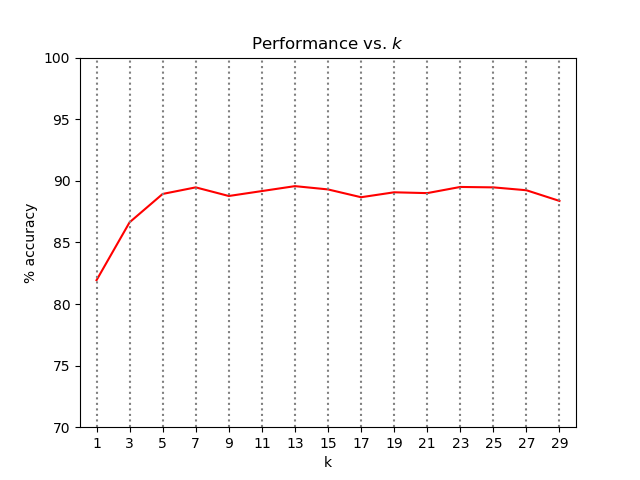
\includegraphics[width=0.9\textwidth]{varying_k.png}
\caption{The accuracy of a kNN classifier on the Sith/Jedi data, as we fiddle
with the number of nearest neighbors used.}
\label{fig:varyingK}
\end{figure}

Real-life data sets normally have more variation than this. Often, there's an
optimal range for $k$ that's quite a bit better than values outside that range,
and there's no surefire way to predict what that range will be until you try
it.

In general, though, the big picture is that \textit{as $k$ increases, the
classifier becomes lower-variance and higher-bias.} Can you see why? For low
values of $k$, we're picking the one (or three, or five, or ...) training
points that just happen to be nearest to our new data point. That's going to be
a lot different depending on which points happen to be in the training set. But
if $k$ is, say, 99, then no matter what training set we get, we're going to
classify most points the same. Like the simple ``just go based on lightsaber
color'' classifier described on p.~\pageref{simpleClassifierTable}, too many
different things would have to simultaneously change between training sets in
order for any different result.


\begin{figure}[ht]
\centering
\begin{Verbatim}[fontsize=\small,samepage=true,frame=single,framesep=3mm]
# Run Naive Bayes, and return the accuracy as a percentage.
def naive_bayes(s):
    train = s.sample(frac=.7)
    test = s.drop(train.index)

    oe = OrdinalEncoder()
    converted_features = oe.fit_transform(train.drop(['type'], axis=1))

    naive_bayes = CategoricalNB()
    naive_bayes.fit(converted_features, train.type)
    nb_predictions = naive_bayes.predict(
        oe.fit_transform(test.drop(['type'], axis=1)))
    return (nb_predictions == test.type).sum() / len(test) * 100


## Run kNN, and return the accuracy as a percentage.
def kNN(s, k):
    train = s.sample(frac=.7)
    test = s.drop(train.index)

    ohe = OneHotEncoder()
    one_hotted_features = ohe.fit_transform(train.drop(['type'], axis=1))

    knn = KNeighborsClassifier(n_neighbors=k)
    knn.fit(one_hotted_features, train.type)
    knn_predictions = knn.predict(
        ohe.fit_transform(test.drop(['type'], axis=1)))
    return (knn_predictions == test.type).sum() / len(test) * 100
\end{Verbatim}

\caption{Two functions, each of which chooses a random 70\% of a data set's
rows for training, runs a classifier on the remaining rows, and returns its
percent accuracy. Note that every time either of these functions is called, a
different answer will be returned, since a new training set will be chosen at
random.}
\label{comparisonCode}
\end{figure}

\section{``The curse of dimensionality''}
\label{sec:curse}

\index{curse@``the curse of dimensionality''}

A second key ML principle goes by the humorous name ``\textbf{the curse of
dimensionality}.'' It goes something like this. Suppose that in addition to
\texttt{height}, \texttt{demeanor}, \texttt{lightsaber}, and \texttt{face}, we
also have at our disposal many other features about Jedi \& Sith: their ages,
salaries, home planets, personality profiles, number of traffic tickets,
\textit{etc.} This is good news, right? It gives us more and more data to sift
through statistically and discover potential correlations with, right? What's
not to like?

\index{data sparsity}
\index{sparsity}

Yes, but there's a catch. It turns out that as we increase the number of
features more and more (or, put another way, as we increase the
``dimensionality'' of the problem from our original four dimensions to 5, 6, 7,
..., and up into the hundreds) we have a \textbf{data sparsity} problem. This
means there aren't enough training points to adequately cover all of this
ground.

In terms of kNN classifiers, you can think of it this way: effectively,
\textit{all} the points become far apart. We want to find the 3 (or 15, or 77)
``nearest neighbors,'' but when we have so many features (many of which will
turn out to be irrelevant for the problem), we find that \textit{any} two data
points will differ on a large number of them. Essentially, our noise swamps our
signal.

When we have tons of features, we need an enormous number of training samples
in order to guarantee that we have several samples with each combination of
values (or their ranges). In our original problem, we didn't need too much data
to ensure that we'd have at least a few \texttt{tall},
\texttt{green}-lightsabered, \texttt{menacing} individuals with a
\texttt{clean} face. But how many training points will we need before we have
several \texttt{tall}, \texttt{green}-lightsabered, \texttt{menacing},
38-year-old, extroverted, abstract-thinking individuals from Tatooine with 4
traffic tickets and a beard who earn 6,000 Galactic credits annually? Answer: a
lot. And if we don't have that many, a kNN classifier trained on all those
features is going to struggle trying to find ``people like this one'' in order
to make a prediction.

\index{feature selection}

The moral to the story is that we will often need to trim our set of features,
sometimes aggressively, if we have too many. It feels wasteful -- all this
great data on all these people, and we're throwing it away! -- but it's the
right thing to do. This process is called \textbf{feature selection}, and
we'll cover it more fully in the next chapter.
% FIX: actually add the feature selection chapter. (lesson 14 from 2019)

\medskip
In the meantime, here are three useful principles for avoiding the curse:

\begin{enumerate}

\item By far the most important thing to recognize is that if you have
additional features that are \textit{truly} correlated with the target -- and
don't simply repeat information contained in the features you already have --
it's okay to include them. Adding more stuff that actually contains useful
information for prediction isn't generally a problem. The problem is when you
add features that are largely \textit{noise}, since they will overwhelm the
truly significant features if there are too many of them.

\item A common rule of thumb is to make sure you have at least \textit{five}
training points for each combination of feature values. (In our Jedi example,
with three \texttt{height}s and three \texttt{lightsaber} values and two
values for the other features, this would imply a training set of at least $(3
\times 3 \times 2 \times 2) \times 5 = 180$ training points.)

\index{parametric model}

\item When the size of the training set becomes too small, use
\textbf{parametric} methods (like Na\"{i}ve Bayes or linear regression) rather
than instance-based methods (like kNN) because they suffer less from the curse.

\end{enumerate}


